\chapter{\ifenglish Introduction\else ข้อมูลทั่วไปของบรษัท\fi}

\section{\ifenglish Company History\else ประวัติความเป็นมาของบริษัท\fi}

SCB TechX \cite{techxWebsite} ก่อตั้งขึ้นจากความร่วมมือระหว่าง SCBX กลุ่มธุรกิจการเงินและเทคโนโลยีชั้นนำของไทย และ Publicis Sapient บริษัทที่ปรึกษาด้านดิจิทัลทรานส์ฟอร์เมชันระดับโลก มีจุดมุ่งหมายเพื่อมอบบริการด้านเทคโนโลยีที่ตอบสนองความต้องการของธุรกิจต่าง ๆ ตั้งแต่การสร้างนวัตกรรมและผลิตภัณฑ์ใหม่ ไปจนถึงการนำเทคโนโลยีมาเพิ่มประสิทธิภาพในการดำเนินงาน

บริษัทมีความเชี่ยวชาญในการพัฒนาโซลูชันในระดับองค์กร (Enterprise-grade solutions) ที่ปลอดภัยและรองรับการใช้งานของฐานลูกค้าจำนวนมาก นอกจากนี้ SCB TechX ยังจัดองค์กรในรูปแบบ Startup เพื่อลดความซ้ำซ้อนในการทำงานและส่งเสริมความคิดริเริ่มใหม่ ๆ ทำให้สามารถพัฒนาโซลูชันให้กับลูกค้าได้อย่างรวดเร็วและมีประสิทธิภาพ


\section{\ifenglish Company Product\else บริการและผลิตภัณฑ์ของบริษัท\fi}
SCB TechX นำเสนอนวัตกรรมที่พร้อมใช้งานหลากหลายด้าน \cite{techxProduct} ทั้งระบบยืนยันตัวตนแบบดิจิทัลด้วยระบบ KYC \cite{whatIsKYC} ซึ่งทางบริษัทจะเรียกว่า eKYC และแพลตฟอร์มทางการเงินที่หลากหลาย นวัตกรรมเหล่านี้สามารถเชื่อมต่อกับระบบของลูกค้าได้อย่างรวดเร็วและง่ายดาย พร้อมทั้งปรับแต่งตามความต้องการเฉพาะของธุรกิจ ส่งผลให้ลูกค้าของ SCB TechX สามารถเปิดตัวบริการใหม่หรือยกระดับการให้บริการได้อย่างทันท่วงที

นอกจากนี้ SCB TechX ยังให้บริการที่ครอบคลุมด้านการให้คำปรึกษาทางเทคโนโลยี (Technology Consulting), โซลูชันด้านโครงสร้างพื้นฐานและแพลตฟอร์ม (Infrastructure \& Platforms), โซลูชันคลาวด์ (Cloud Solutions), แพลตฟอร์มเทคโนโลยีแบบครบวงจร (xPlatform), การจัดการข้อมูลและความปลอดภัย (Data \& Security), และโซลูชันด้านข้อมูลและ AI (TechX Data \& AI Solutions) ที่ออกแบบมาเพื่อรองรับและเสริมสร้างศักยภาพให้กับธุรกิจในยุคดิจิทัล

\clearpage

\section{\ifenglish Organization\else ผู้บริหารของบริษัท\fi}
\begin{table}[ht]
    \centering
    \begin{tabular}{|c|c|}
        \hline
        \textbf{Name}          & \textbf{Position}            \\
        \hline
        Trirat Suwanprateeb    & Chief Executive Officer      \\
        Jonathan Sharp         & Chief Technology Officer     \\
        Pavarej Hwangdee       & Chief Product Officer        \\
        Yuwanan Buranaanusorn  & Chief Finance Officer        \\
        Jaruwan Lueponglukkana & Chief Human Resource Officer \\
        \hline
    \end{tabular}
    \caption{Company Leadership}
\end{table}
\begin{figure}[ht]
    \begin{center}
        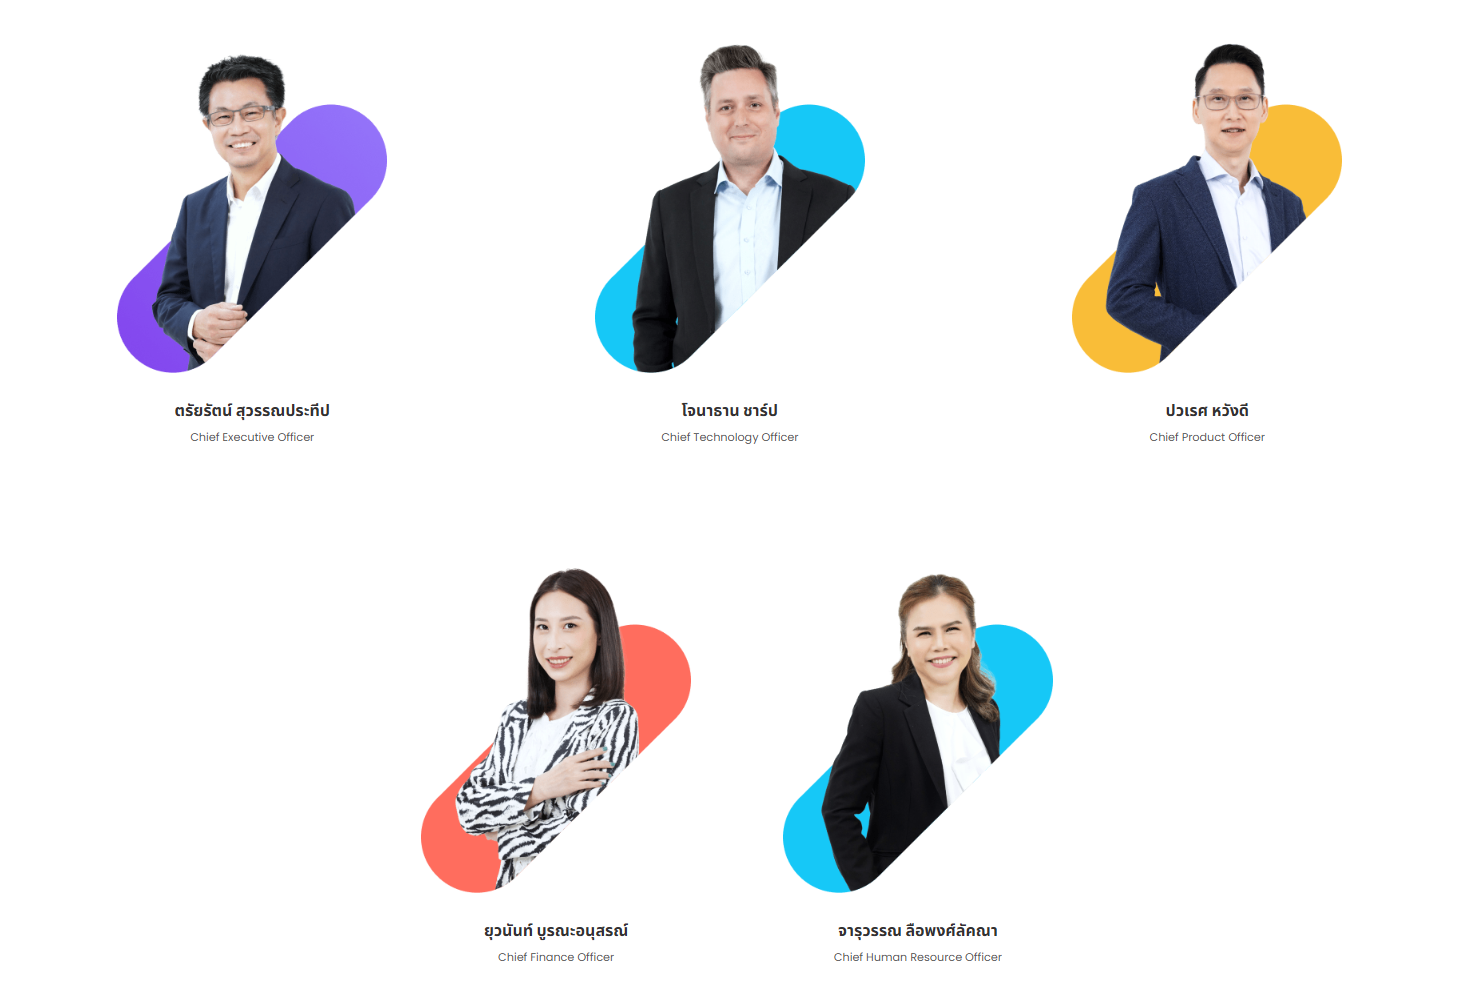
\includegraphics[scale=0.3]{images/org.png}
    \end{center}
    \caption[ผู้บริหารและตำแหน่งของบริษัท]{ผู้บริหารและตำแหน่งของบริษัท}
\end{figure}

\clearpage

\section{หน้าที่ของหน่วยงานที่ได้มาสหกิจ}
ในตำแหน่ง DevOps Engineer ที่ SCB TechX หน้าที่หลักของผมคือการทำงานเป็นตัวกลางระหว่างทีมพัฒนา (Development Team) และทีมปฏิบัติการ (Operation Team) โดยมุ่งเน้นไปที่การพัฒนาและจัดหาเครื่องมือเพื่อช่วยในการบริหารจัดการระบบ รวมถึงสนับสนุนการทำงานของทีมพัฒนา นอกจากนี้ ยังมีบทบาทสำคัญในการดูแลและปรับปรุงกระบวนการ CI/CD เพื่อให้การส่งมอบระบบไปยังผู้ใช้ (Delivery) เป็นไปอย่างราบรื่นและรวดเร็ว

ในด้านอื่น ๆ ผมยังมีหน้าที่ในการเตรียมความพร้อมของ Pipeline สำหรับการ Deploy และสร้างเครื่องมืออัตโนมัติ (Automation Tools) เพื่อช่วยลดเวลาทำงานของทุกทีมในองค์กร อีกทั้งยังทำหน้าที่ประสานงานเกี่ยวกับเครือข่าย (Network) และความปลอดภัย (Security) เพื่อสนับสนุนทีมอื่น ๆ ภายในบริษัทตามขอบเขตงานที่ได้รับมอบหมาย

% \section{\ifenglish Objectives\else วัตถุประสงค์ของรายงาน\fi}
% \begin{enumerate}
%     \item
% \end{enumerate}

% \section{\ifenglish Project scope\else ขอบเขตของรายงาน\fi}

% \subsection{\ifenglish Hardware scope\else ขอบเขตด้านฮาร์ดแวร์\fi}

% \subsection{\ifenglish Software scope\else ขอบเขตด้านซอฟต์แวร์\fi}

% \section{\ifenglish Expected outcomes\else ประโยชน์ที่ได้รับ\fi}

% \section{\ifenglish Technology and tools\else เทคโนโลยีและเครื่องมือที่ใช้\fi}

% \subsection{\ifenglish Hardware technology\else เทคโนโลยีด้านฮาร์ดแวร์\fi}

% \subsection{\ifenglish Software technology\else เทคโนโลยีด้านซอฟต์แวร์\fi}

% \section{\ifenglish Project plan\else แผนการดำเนินงาน\fi}

% \begin{plan}{6}{2020}{2}{2021}
%     \planitem{7}{2020}{8}{2020}{ศึกษาค้นคว้า}
%     \planitem{8}{2020}{1}{2021}{ชิล}
%     \planitem{2}{2021}{2}{2021}{เผา}
%     \planitem{12}{2019}{1}{2022}{ทดสอบ}
% \end{plan}

% \section{\ifenglish Roles and responsibilities\else บทบาทและความรับผิดชอบ\fi}
% อธิบายว่าในการทำงาน นศ. มีการกำหนดบทบาทและแบ่งหน้าที่งานอย่างไรในการทำงาน จำเป็นต้องใช้ความรู้ใดในการทำงานบ้าง

% \section{\ifenglish%
% Impacts of this project on society, health, safety, legal, and cultural issues
% \else%
% ผลกระทบด้านสังคม สุขภาพ ความปลอดภัย กฎหมาย และวัฒนธรรม
% \fi}

% แนวทางและโยชน์ในการประยุกต์ใช้งานรายงานกับงานในด้านอื่นๆ รวมถึงผลกระทบในด้านสังคมและสิ่งแวดล้อมจากการใช้ความรู้ทางวิศวกรรมที่ได้
